
\section{Introduction}
%This paper uses the task of hitting a point target precisely with a whip as a case study for dynamic manipulation of deformable object. 
We study the task of goal-conditioned dynamic manipulation of deformable objects, examples of which include whipping a target point with the tip of a rope or spreading a cloth into a target pose (Fig. \ref{fig:teaser}). 
Humans show remarkable ability to not only perform these tasks with high precision (e.g., aiming a lasso or setting a table cloth), but also to quickly transfer these manipulation skills to new objects with very few attempts. 
For robots, however, this has historically been a highly challenging problem due to several factors:

\begin{itemize}[leftmargin=3mm]
\item \textbf{Complex dynamics:} Unlike quasi-static manipulation, dynamic manipulations (often with high-speed actions) often lead to complex and non-linear effects. 
% These dynamical processes are difficult to model and sensitive to measurement errors and initial conditions. 
These dynamical processes are difficult to model, and pose significant challenges for system identification and state estimation.
As a result, it is often infeasible to apply classical algorithms, such as optimal control, when an accurate and performant forward model of the system is prohibitively difficult to obtain.

\item \textbf{Complex object properties:} 
Unlike rigid objects, deformable objects exhibit dynamics that are influenced by numerous hard-to-estimate factors such as nonlinear anisotropic stiffness, friction, density distribution, and changing aerodynamics. Not only is it challenging to estimate these properties, it is hard to map them to the parameter used in common simulators using simplified physics models.

% Unlike a rigid object, the motion of a deformable object is influenced by numerous factors that are difficult to both measure and simulate such as stiffness, aerodynamics, and density distribution. These factors, coupled with the high degree of freedom that deformable objects posses, result in a significant sim2real gap inherent in the simulation of deformable objects.


% As a result, classical algorithms such as model-based control and iterative learning control fail to produce satisfying results. 
%Instability of this dynamic system makes trajectory prediction sensitive to modeling error, measurement error and initial condition error. Several classes of classical algorithms such as model-based control and iterative learning control produce underwhelming result.

\item \textbf{Precise goal conditions:}  Due to these challenges, prior work that applies dynamic manipulation to deformable objects generally studies tasks with low precision requirements such as cloth unfolding \cite{ha2021flingbot} or cable vaulting \cite{zhang2021robots}. In contrast, the tasks studied in this paper require precise actions in order to reach the specified goal conditions --- for example hitting a goal location with the tip of a whip or reaching a goal configurations defined by keypoints on a cloth.

\end{itemize}


\begin{figure}[t]
    \centering
    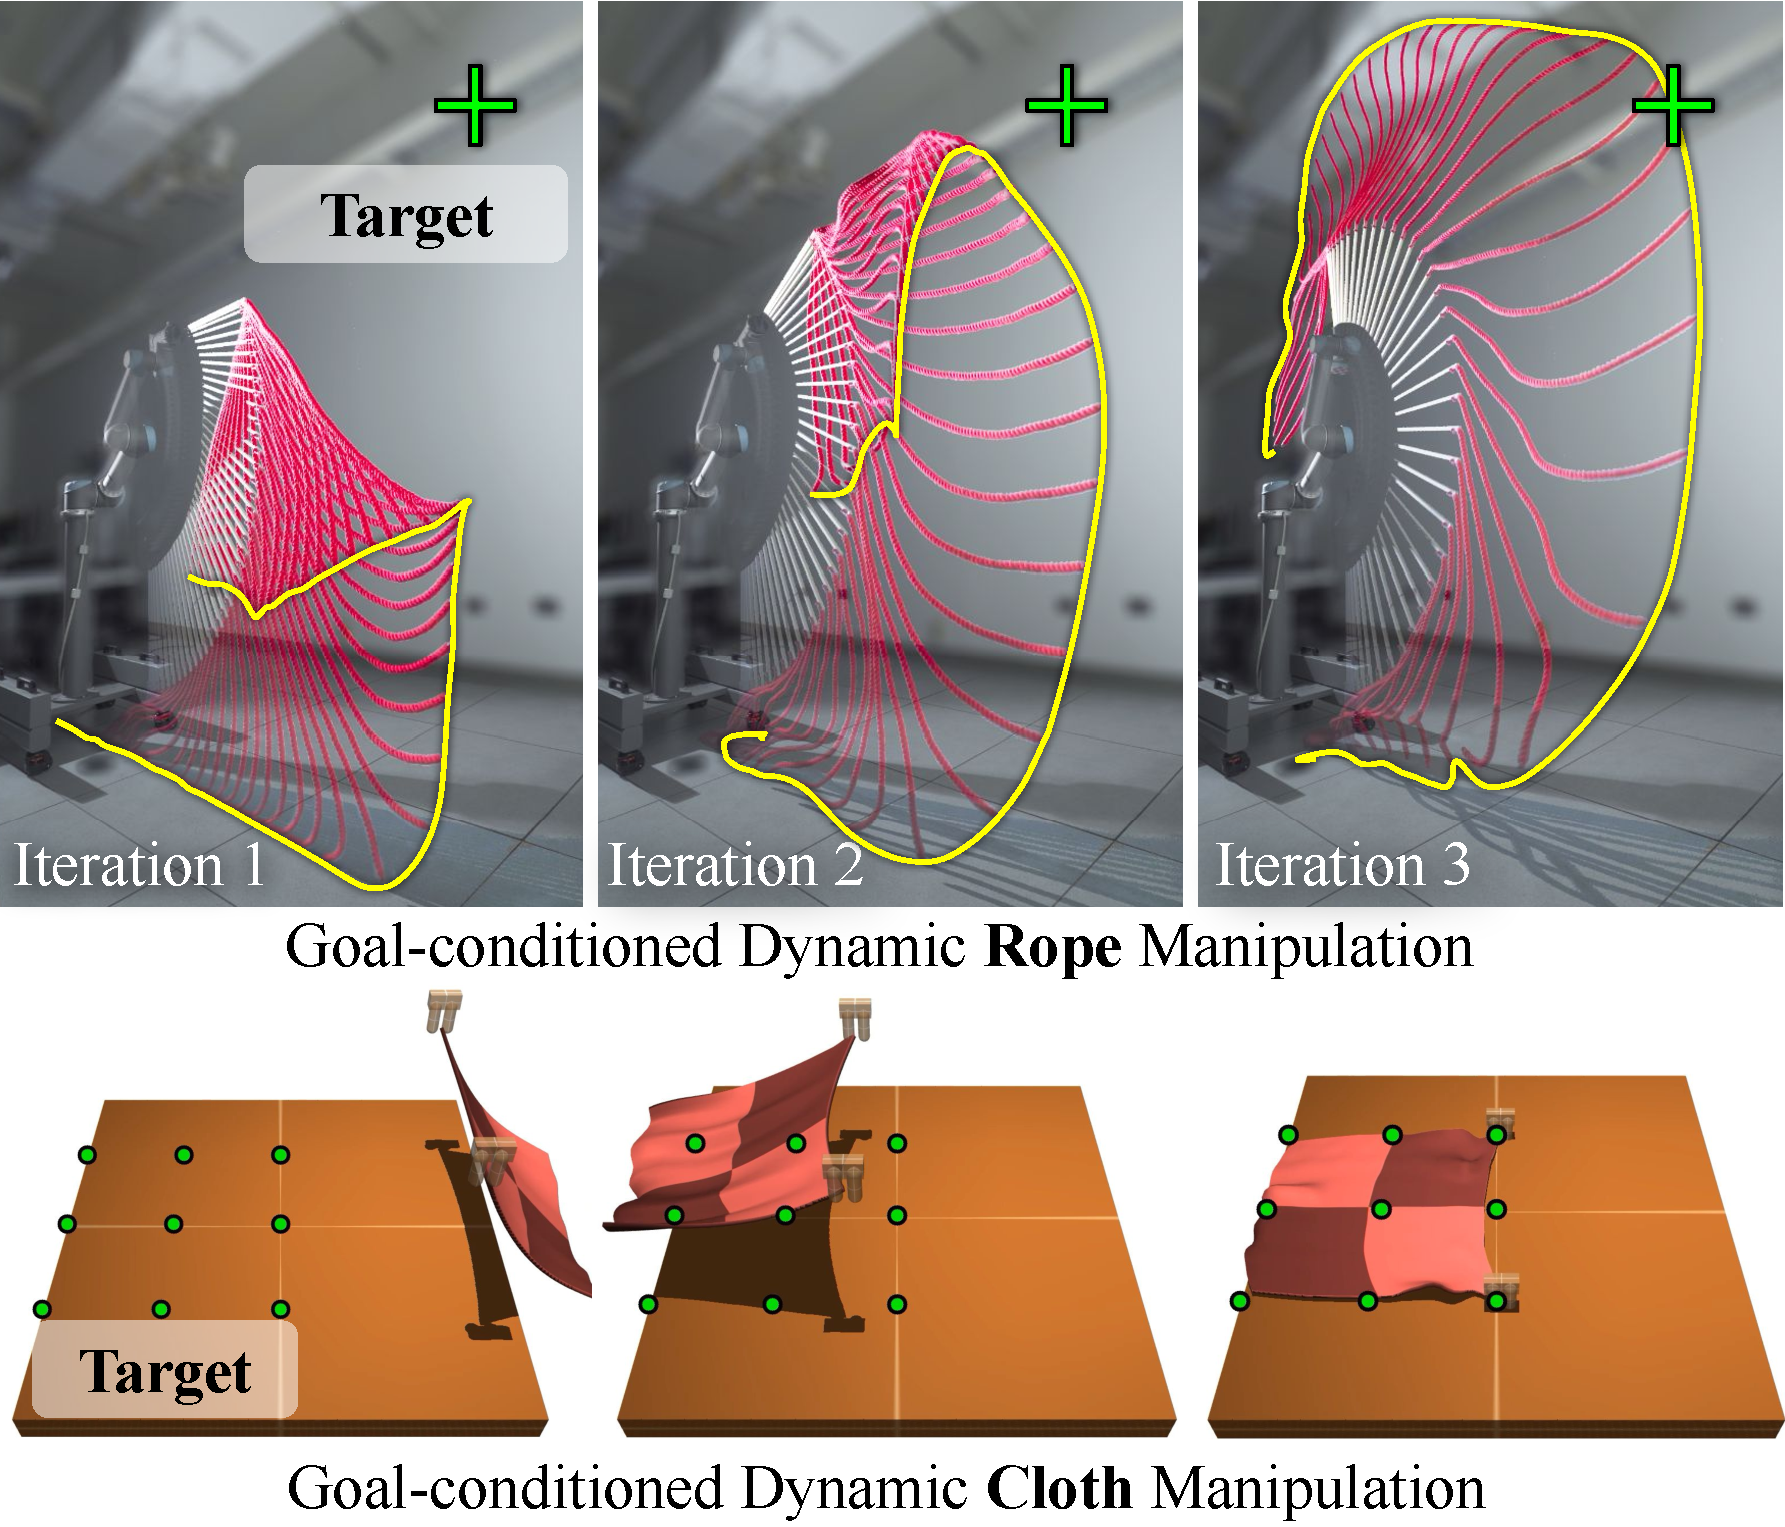
\includegraphics[width=\linewidth]{figure/rope-teaser.pdf}
    %https://docs.google.com/drawings/d/12tlTQ5S-eEHEXbHswpW1-dkgyWmvPPUlsDF5sNXWmwo/edit?usp=sharing
    \caption{\textbf{Goal-conditioned dynamic manipulation of deformable objects.}  Our method achieves high accuracy by iteratively adjusting actions using visual feedback and a learned delta dynamics network. Top: Rope manipulation task. Goal configuration is defined by a target tip position (green cross).  Bottom: Cloth manipulation task. Goal configuration is defined by target keypoint locations (green dots). }
    \vspace{-5mm}
    \label{fig:teaser}
\end{figure}


To address these challenges, we present \textbf{\namel~(\names)}, a general formulation for goal-conditioned dynamic manipulation, that learns how to iteratively improve its actions to achieve a given goal condition using visual feedback.
This formulation highlights two key features: 

\begin{figure*}[t]
    \centering
    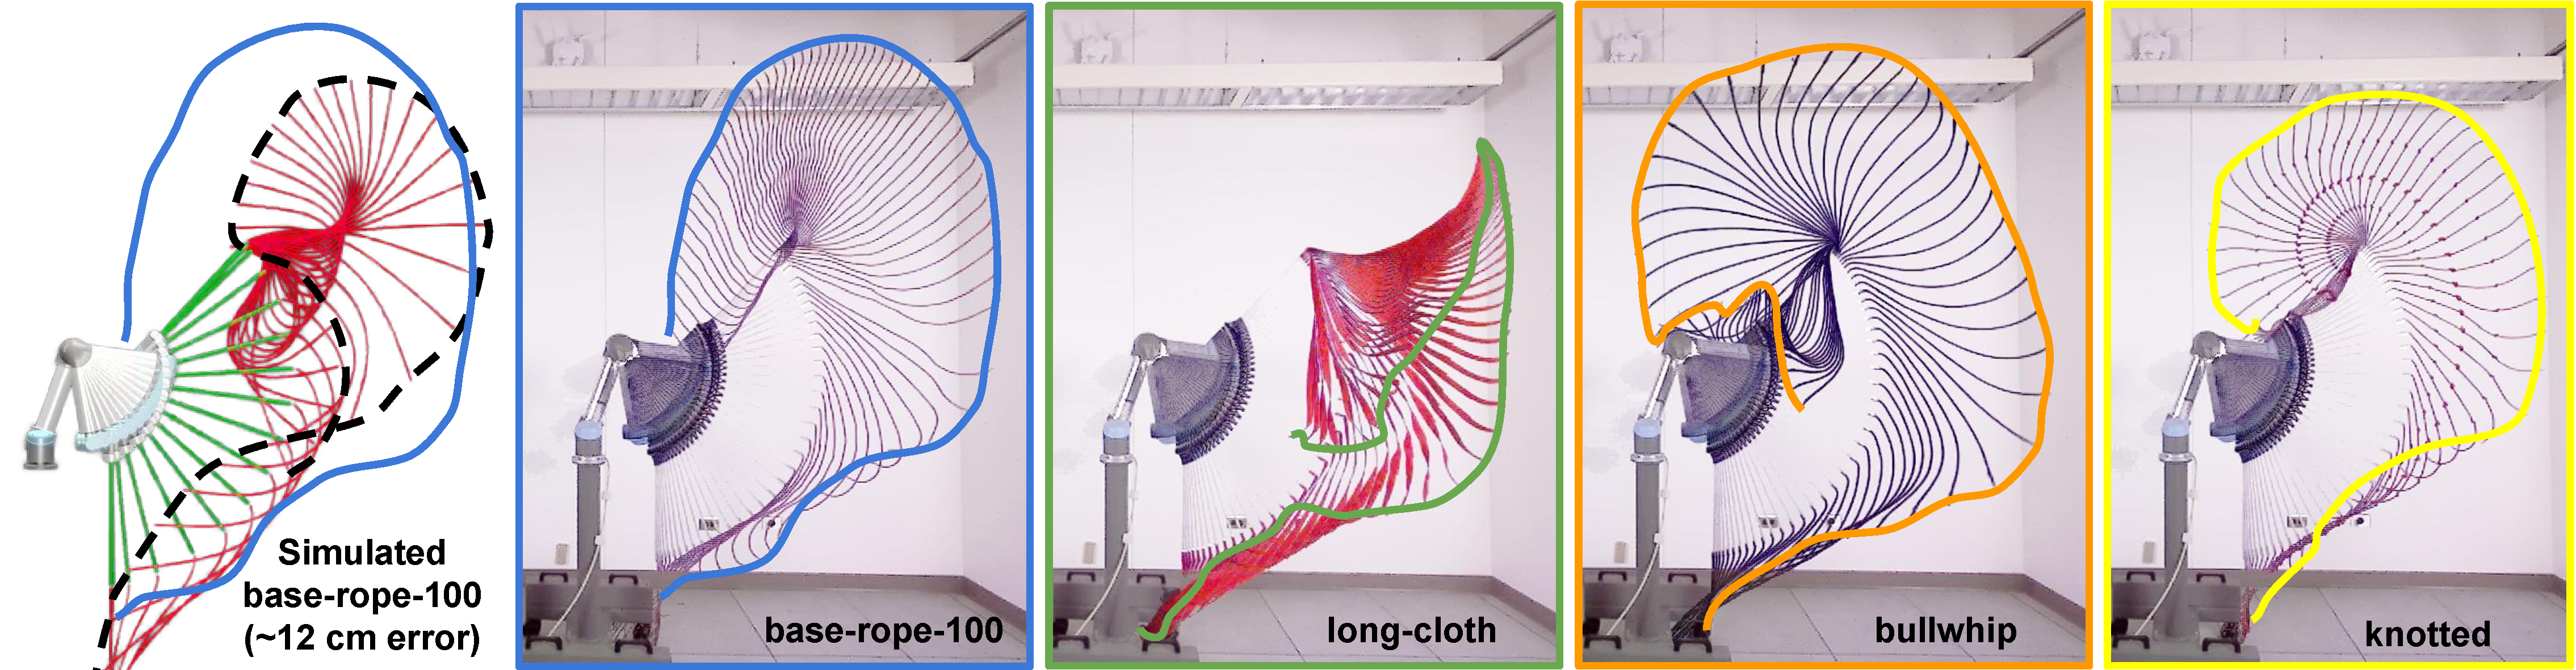
\includegraphics[width=\linewidth]{figure/rope-challenge.pdf}
    \caption{\textbf{Challenges.} Here we show the different rope trajectories under the \textbf{same} robot action. Due to different physical properties (e.g., aerodynamic, mass distribution or stiffness), the resulting trajectories varies drastically. Left plot shows the trajectory overlay between the real-world (solid curve) and simulated result (dashed curve) both for base-rope-100. The offset between them indicates the sim2real gap even with the accurate rope parameters.  These examples highlight the importance of online adaptation that is necessary for both sim2real transfer and generalization to novel ropes with unknown parameters. } \vspace{-3mm}
    \label{fig:challenge}
    %https://docs.google.com/drawings/d/1iENSKLm8TAqqpHCGbYWxNpbn4WoV1e2MpJIWHfZ2rrY/edit
    \vspace{-3mm}
\end{figure*}


\begin{itemize}[leftmargin=3mm]
\item \textbf{Iterative action refinement}: Instead of directly inferring the optimal action from the goal, \names~starts with a best guess action and iteratively refines it to move toward the goal. For tasks with repeatable dynamics, this iterative approach allows the system to achieve high precision and be robust against errors from action, observation, and model prediction.

% \item \textbf{Residual trajectory representation}: 
\item \textbf{Delta dynamics}: 
Within each iteration, \names~ learns to predict an updated trajectory from an observed trajectory with small action perturbations. Compared to modeling the entire dynamical system (action in, trajectory out), this ``delta dynamics'' (especially its general direction) is much easier to predict and generalize to new objects, thereby, enabling quick online adaption.  

% \cheng{Instead of modeling the dynamical system from scratch, \names~bootstraps its prediction of the resulting trajectory from small action perturbations using the observed trajectory.}

% Instead of modeling task dynamics from scratch, \names~bootstraps residual dynamics prediction relative to a previously observed trajectory. Given a previously observed trajectory and a set of possible changes to those actions (delta actions), the residual dynamics module predicts the resulting trajectories.
% Since the input trajectory retains the rich information about the object at hand, this formulation allows the model to quickly adapt to new object instances that are not in the training data. 

% Instead of modeling the entire dynamical system, \names~learns to predict the resulting trajectory (spatially represented as a 2D image) of small action perturbations on the observed trajectory.
% To model the system dynamics, \names~learns to predict residual trajectories (spatially represented as a 2D image) of the observed rope trajectory under small perturbations on the current action. 
% Compared to modeling the whole dynamical system, the residual trajectory is much easier to predict, especially when the delta action is small. 
%, without the problem of compounding error.
% \shuran{is is true? wonder why?} 

%This formulation efficiently retains the rich physical information captured by the observation, which allows the model to generalize to unseen ropes with significantly different dynamics comparing to training data. 
%\shuran{still not clear why this formulation better in generalization. Do you want to say delta trajectory is easier to learn than learning the whole dynamical system? e.g., sysid?}

\end{itemize}

Our  primary contribution is the \namel~(\names), a general learning framework for goal-conditioned dynamic manipulation. 
Despite only trained using simulation data, \names~can be directly applied to real-world hardware. Furthermore, \names~demonstrates impressive generalization capability to unseen object instances, out-of-distribution rope parameters, unmodeled physical effects, and varying robot embodiments.
% Thanks to its adaptable formulation, the model trained in simulation can be directly applied to a real-world robot platform without fine tuning.  
Our experiments show that \names~can achieve pixel level accuracy for a wide variety of goals in both simulation and real robot environments (1.8cm and 2.6cm respectively).
% \todo{update experiment result reflect both tasks}. 
% In particular, our method maintains the same level of accuracy while generalizing to out-of-distribution rope parameters, unmodeled physical effects and varying robot embodiments.


% \textbf{Problem:}
% \begin{itemize}    
%     \item{Difficult to model dynamics}: High degrees of freedom with non-linear dynamics and difficult to measure parameters. \textbf{Hard to compute Jacobian analytically.} This makes model-based control/RL difficult. \textbf{Large sim-to-real gap.}
    
%     \item{Difficult to plan/control}: Highly underacutated. Goal can not be mapped trivially to actions.
% \end{itemize}

% \textbf{Solution:}
% \begin{itemize}
%     \item{Learning the notion of Jacobian} for \textbf{online adaptation}. Intuitive physics.
%     \item{Identical input and output representation} easier to learn, better generalization.
%     \item{Motion primitive} to reduce action space.
% \end{itemize}

% \textbf{Contribution:}
% \begin{itemize}
%     \item{First to solve a task} Goal conditioned dynamic manipulation of deformable.
%     \item{A method to close the sim-to-real gap} Representation to enable online adaptaion.
% \end{itemize}

% \textbf{Key takeaway:}
% \begin{itemize}
%     \item{Learned close-loop policy transfer better}
%     \item{Decouple goal and learning}
%     \item{}
% \end{itemize}


% Current literature interpreters the term intuitive physics in different ways. 
% 1. Object permance
% 2. Learning output of physics simulation or residual
% 3. Predict next state given current state and action

% Our work is more in-line with clever reformulation of the original problem for easier learning.
% And turn problem into class 3.
